%!TeX root=../tese.tex
%("dica" para o editor de texto: este arquivo é parte de um documento maior)
% para saber mais: https://tex.stackexchange.com/q/78101/183146

%% ------------------------------------------------------------------------- %%
\chapter{Introdução}
\label{cap:introducao}

%[Em geral a introdução é algo que procura ser atraente, motivacional e elementar.]

De tempos pra cá, ler e ouvir falar de ciência de dados tornou-se muito comum, tanto nos meios profissionais e científicos quanto na mídia. Existem atualmente aplicações em praticamente todas as áreas do conhecimento humano, da agricultura à indústria e ao entretenimento.

Joel Grus \citep{data} define genericamente \defi{ciência de dados} como sendo a extração de conhecimento a partir de dados desorganizados. Os dados podem ser números, textos, áudio, vídeo, entre outros quaisquer que podem ser úteis na tomada de decisões de negócios.

Pedro A. Morettin e Julio M. Singer \citep{apostila} afirmam que este termo, embora usado como se fosse um conceito novo, não está separado dos conceitos já históricos da \emph{estatística}. Eles apontam que o trabalho dos \emph{cientistas de dados} difere do trabalho dos \emph{estatísticos} apenas quando eles usam dados multimídia como áudio, vídeo, ou textos. Mas que, uma vez que esses dados são processados e tornam-se números, as técnicas e conceitos utilizados por ambos passam a ser basicamente os mesmos.

Na verdade, Morettin e Singer \citep{apostila} citam que na década de 80 houve uma primeira tentativa de aplicar o rótulo \emph{ciência de dados}, (\emph{Data Science}), ao trabalho feito pelos estatísticos aplicados da época, como uma forma de dar-lhes mais visibilidade. Curiosamente, fato mencionado pelos autores, existem atualmente cursos específicos de ciência de dados em universidades ao redor do mundo, mas a maioria deles situada em institutos de áreas aplicadas como engenharia e economia, e raramente nos institutos de estatística propriamente ditos.

Para entender um pouco mais de seu escopo, David M. Blei e Padhraic Smyth \citep{blei} discutem ciência de dados sob as visões estatística, computacional e humana. Eles argumentam que é a combinação desses três componentes que formam a essência do que ela é e, assim como, do conhecimento que ela é capaz de produzir.

Pode-se extender e observar essa ideia de uma visão em conjunto dos aspectos estatísticos, computacionais e humanos com um diagrama de Venn. Por exemplo, seja o diagrama criado por Andrew Silver \citep{venn} e mostrado a seguir na figura \ref{fig:venn}.

\begin{figure}[htb]
\centering
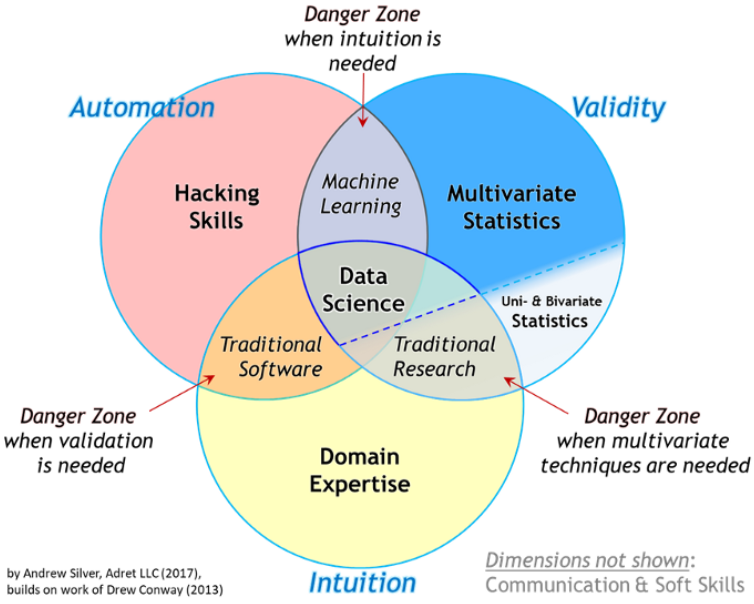
\includegraphics[width=8cm]{figuras/venn}
\caption{Diagrama de Venn relacionando os três aspectos inerentes à ciência de dados.\footnote{Extraído de \citep{venn}}}
\label{fig:venn}
\end{figure}

Dessa forma vemos que no aspecto estatístico, seja univariado ou multivariado, está a criação e validação dos modelos utilizados. No aspecto computacional estão as habilidades computacionais, de criação e de eficiência dos modelos. E que no aspecto humano, está a intuição e o domínio do assunto que está sendo estudado.

Além disso, podemos ver, nas intersecções entre os aspectos, as definições de outros conceitos-chave. O \defi{aprendizado de máquina} está na intersecção entre a estatística e a computação, já que o objetivo é criar modelos \emph{computacionais} a partir de modelos estatísticos. 

Uma pesquisa tradicional utiliza o conhecimento de um profissional da área aliado com habilidades e ferramentas estatísticas. Um software tradicional, por sua vez, é criado por profissionais de tecnologia para o uso de profissionais de outras áreas. 

A ciência de dados, portanto, é a junção desses aspectos, aliando modelagem estatística, automação computacional, validade, e intuição. As áreas perigosas mostradas na figura \ref{fig:venn}, refletem o que pode ocorrer quando algum dos três aspectos é negligenciado numa empreitada de ciência de dados.

Algoritmos de \emph{aprendizado de máquina} vem sendo utilizados em grande parte dos modelos de ciência de dados. Mas o que é aprendizado de máquina? Ou então, o que significa dizer que o computador, neste caso a ``máquina'', está \emph{aprendendo}?

Aurélien Géron \citep{hands} nos dá uma ideia geral lembrando que uma das primeiras aplicações de sucesso de aprendizado de máquina foi o filtro de \eng{spam}, criado na década de 90. Uma das fases de seu desenvolvimento foi aquela em que os usuários assinalavam que certos e-mails eram \eng{spams} e outros não eram. Hoje em dia, raramente temos que marcar ou desmarcar e-mails, pois a maioria dos filtros já ``aprenderam'' a fazer seu trabalho de forma muito eficiente, não temos mais nada a ``ensiná-lo''.

O conceito de aprendizado de máquina está intimamente ligado à ciência da computação. Porém, no contexto de ciência de dados, é definido por Grus \citep{data} como a ``criação e o uso de modelos que são ajustados a partir dos dados''. Seu objetivo é usar dados existentes para desenvolver modelos que possamos usar para \emph{prever} possíveis respostas à consultas. 

Exemplos, além do filtro de \eng{spams} podem ser: detectar transações de crédito fraudulentas, calcular a chance de um cliente clicar em uma propaganda ou então prever qual time de futebol irá vencer o Campeonato Brasileiro.

Como ficará claro ao longo deste trabalho, o aprendizado consiste na utilização de dados já conhecidos para ajustar parâmetros de modelos. Uma vez ajustados os parâmetros, o algoritmo que descreve o modelo passa a ser usado para responder às consultas. Essa fase de ajuste de parâmetros é chamada de aprendizado ou treinamento. 

Uma \defi{rede neural} é um exemplo de modelo preditivo de aprendizado de máquina que foi criado com inspiração no funcionamento do cérebro biológico. David Kopec \citep{classic} descreve que apesar de terem sido as primeiras a serem criadas, elas vem ganhando nova importância na última década, graças ao avanço computacional, uma vez que exigem muito processamento, e também porque podem ser usadas para resolver problemas de aprendizagem dos mais variados tipos.

Atualmente existem vários tipos de redes neurais, porém este trabalho lida principalmente com aquele tipo que foi originalmente criado sob a inspiração do funcionamento do cérebro, chamado de \defi{perceptron}, e que portanto tenta imitar o comportamento dos neurônios e suas conexões, aprendendo padrões a partir de dados existentes e tentando prever o comportamento de dados novos a partir do padrão aprendido.

Uma visão geral da arquitetura do aprendizado de máquina, situando a posição das redes neurais e do algoritmo \eng{perceptron} em toda esta estrutura, assim como exemplos de aplicações em cada uma das suas ramificações, estão no Capítulo \ref{cap:redes}.

Neste trabalho é utilizada como base didática uma versão simples do algoritmo \eng{perceptron} feita e explicada por Kopec \citep{classic}, e a partir desta base, foram criados novos métodos de treinamento e de validação com algumas estratégias, como uma tentativa de automatizar e otimizar o processo de treinamento do algoritmo, que é comumente feito de forma heurística. Detalhes dessa implementação estão no Capítulo \ref{cap:perceptron}.

São apresentados os conceitos e usos das séries temporais de dados não-lineares no Capítulo \ref{cap:series}, assim como alguns exemplos de aplicações na área financeira. As técnicas tradicionais de análise e de previsão de séries temporais de dados serão brevemente apresentadas neste capítulo.

Para servir de validação e aplicação do algoritmo criado, no Capítulo \ref{cap:comparacao} serão feitas comparações de desempenho entre o \eng{perceptron} e os modelos tradicionais de previsões de séries temporais apresentados no capítulo anterior, como o \defi{SARIMA} (\eng{seasonal auto regressive integrated moving average}). Tais comparações usam como inspiração trabalhos similares como o de Alsmadi, Omar, Noah e Almarashdah \citep{4809024}.

Ao final concluo sobre os modelos de previsões aqui estudados e comparados, destacando a qualidade e eficiência dos métodos de redes neurais, tão bons e às vezes melhores do que os métodos tradicionais estatísticos.

